\documentclass{article}

% Packages
\usepackage{hyperref} 
\usepackage[utf8]{inputenc}
\usepackage{lmodern}  % for bold teletype font
\usepackage{amsmath}  % for \hookrightarrow
\usepackage{xcolor}   % for \textcolor
\usepackage{listings}
\usepackage[a4paper, total={6in, 8in}]{geometry}
\usepackage{graphicx}
\usepackage{textcomp}
\usepackage[T1]{fontenc}
\usepackage{hyphenat}
\usepackage[flushleft]{threeparttable}


\lstset{
    upquote=true,
    breaklines=true,
    postbreak=\mbox{\textcolor{red}{$\hookrightarrow$}\space},
}

\title{\textbf{Daily Report File for the Semester Project}}
\author{Furkan Karakaş}

\begin{document}

\maketitle

\section*{9 February 2020}

I did the first installation. I also forked the tendermint repository to my 
GitHub repository \url{https://github.com/FurkanKarakas/tendermint}. We can run a single node tendermint at the moment but to run local testnets, we can utilize \textit{docker}. To start a 4 node testnet, run:

\begin{lstlisting}
make localnet-start
\end{lstlisting}

After executing multiple nodes, a new folder \texttt{build} is created. In this folder, each node has a log file, which is called \texttt{tendermint.log}. These log files contain the commit and execute steps of the program, written with their corresponding timestamps.

The nodes bind their RPC servers to ports 26657, 26660, 26662, and 26664 on the host.
This file creates a 4-node network using the localnode image.
The nodes of the network expose their P2P and RPC endpoints to the host machine on ports 26656-26657, 26659-26660, 26661-26662, and 26663-26664 respectively.

To stop and restart the environment, one can use the following commands:

\begin{lstlisting}
make build-linux
make localnet-stop
make localnet-start
\end{lstlisting}

\section*{20 February 2020}

We need to simulate network delays and packet losses in the Docker containers. There is a very good article here about it: \url{https://alexei-led.github.io/post/pumba_docker_netem/}. Linux allows us to manipulate the traffic flow using a tool called \texttt{tc}, which is available in \texttt{iproute2}. Another tool called \texttt{netem} is an extension of it. It allows us to emulate network failures such as delay, packet loss, packer reorder, duplication, corruption, and bandwidth rate.

For controlling traffic flow in the Docker containers, we will be using a software called \textit{pumba}, which utilizes Linux traffic control and network emulation softwares \textit{tc} and \textit{netem}, respectively. A good documentation of it could be found at the website \url{https://github.com/alexei-led/pumba}.

\begin{figure}
    \centering
    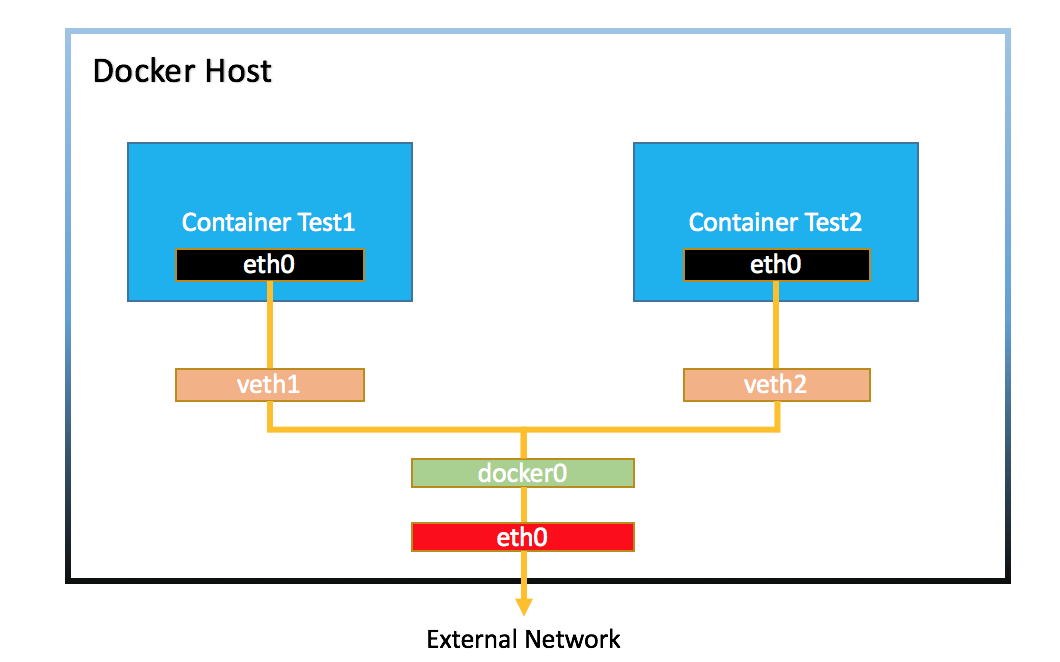
\includegraphics[width=\linewidth]{Pictures/docker_interfaces.png}
    \caption{The basic network topology inside a Docker host}
    \label{fig:interfaces}
\end{figure}

Figure \ref{fig:interfaces} illustrates the basic topology of a Docker host. Basically, \texttt{veth} interfaces are used in order to create a communication between each container and the docker itself. As I type the \texttt{ifconfig} command in the command line, I am able to see the aforementioned virtual interfaces, each corresponding to $node_i$ where $i \in \{0,1,2,3\}$:

\begin{lstlisting}[basicstyle=\small]
veth282987a: flags=4163<UP,BROADCAST,RUNNING,MULTICAST>  mtu 1500
        inet6 fe80::dc1b:3cff:fe06:7484  prefixlen 64  scopeid 0x20<link>
        ether de:1b:3c:06:74:84  txqueuelen 0  (Ethernet)
        RX packets 94167  bytes 57527418 (57.5 MB)
        RX errors 0  dropped 0  overruns 0  frame 0
        TX packets 94874  bytes 58402540 (58.4 MB)
        TX errors 0  dropped 0 overruns 0  carrier 0  collisions 0

veth454c67a: flags=4163<UP,BROADCAST,RUNNING,MULTICAST>  mtu 1500
        inet6 fe80::24fd:25ff:fee5:45f  prefixlen 64  scopeid 0x20<link>
        ether 26:fd:25:e5:04:5f  txqueuelen 0  (Ethernet)
        RX packets 95109  bytes 58670384 (58.6 MB)
        RX errors 0  dropped 0  overruns 0  frame 0
        TX packets 95470  bytes 58291946 (58.2 MB)
        TX errors 0  dropped 0 overruns 0  carrier 0  collisions 0

vethba77776: flags=4163<UP,BROADCAST,RUNNING,MULTICAST>  mtu 1500
        inet6 fe80::b0e9:54ff:fe9d:52cb  prefixlen 64  scopeid 0x20<link>
        ether b2:e9:54:9d:52:cb  txqueuelen 0  (Ethernet)
        RX packets 95284  bytes 58311392 (58.3 MB)
        RX errors 0  dropped 0  overruns 0  frame 0
        TX packets 94967  bytes 58303854 (58.3 MB)
        TX errors 0  dropped 0 overruns 0  carrier 0  collisions 0

vethe97798a: flags=4163<UP,BROADCAST,RUNNING,MULTICAST>  mtu 1500
        inet6 fe80::4c55:84ff:fe93:4da8  prefixlen 64  scopeid 0x20<link>
        ether 4e:55:84:93:4d:a8  txqueuelen 0  (Ethernet)
        RX packets 94980  bytes 58487742 (58.4 MB)
        RX errors 0  dropped 0  overruns 0  frame 0
        TX packets 95391  bytes 58199768 (58.1 MB)
        TX errors 0  dropped 0 overruns 0  carrier 0  collisions 0

\end{lstlisting}

Following is a simple command to delay the traffic at \texttt{node0} 20 seconds with a duration of 30 seconds:

\begin{lstlisting}
sudo pumba netem --duration 30s --interface eth0 --tc-image 'gaiadocker/iproute2' delay --time 20000 node0
\end{lstlisting}

\section*{27 February 2020}

We need some network emulation techniques to test the tendermint under various conditions, including but not limited to:

\begin{itemize}
    \item network delays by an arbitrary amount of time including jitter,
    \item network packet loss while sending packets from one node to another,
    \item packet duplication,
    \item corrupt packets,
    \item process crashes under different models, e.g., crash-recovery, crash-stop, etc.
\end{itemize}

We can emulate those behaviours by means of the \texttt{pumba} software, which is basically a toolbox for stress testing the docker containers.

In order to send transactions to the nodes, we can utilize the following command:

\begin{lstlisting}
curl -s 'localhost:{NODE_PORT}/broadcast_tx_commit?tx="{TX_NAME}"'
\end{lstlisting}

where \texttt{NODE\_PORT} is the RPC port of the nodes that participate in the algorithm, and \texttt{TX\_NAME} is the name of the transaction that we would like to send. After sending a transaction, each participating node attests that this was a valid transaction in an \textit{executed block}, then commits these changed in a \textit{committed state}. After committing, the value of the \texttt{appHash} in the nodes also changes, where \texttt{appHash} is a hexadecimal number. For example, at start, the value of \texttt{appHash} was \texttt{appHash=0000000000000000}. After sending the transaction successfully, it became \texttt{appHash=0200000000000000}, after another transaction, \texttt{appHash=0400000000000000}, etc. Each participating node printed the following text after a successful transaction individually:

\begin{lstlisting}
I[2020-02-27|10:08:48.317] Executed block  module=state height=6183 validTxs=1 invalidTxs=0

I[2020-02-27|10:08:48.319] Committed state module=state height=6183 txs=1 appHash=0400000000000000
\end{lstlisting}

Hence, this transaction is registered in the blockchain at height 6183.

Using network delays, I tried to send a transaction. With a network delay of 5000 ms, it took a while to validate the transaction, but at the end, the transaction is eventually validated by every participating node in the algorithm.

I created appropriate bash scripts for the stress testing of the Docker containers.  From time to time, when I use the network emulation commands, e.g., when I try to simulate packet duplication, I get the following error from various nodes:

\begin{lstlisting}
node2    | E[2020-02-27|13:35:05.265] dialing failed (attempts: 1): self ID<fa97dbb3d7afd62fa818f9a535fc88ed54fc283c> module=pex addr=fa97dbb3d7afd62fa818f9a535fc88ed54fc283c@192.167.10.4:26656

\end{lstlisting}

Currently, I created a bash script for sending successive transactions to a node.

\section*{5 March 2020}

We can also send a key-value pair to the program. We observe that in the HTTP response, we have only the key in the JSON format:

\begin{lstlisting}
{
  "key": "Y3JlYXRvcg==",
  "value": "Q29zbW9zaGkgTmV0b3dva28="
},
{
  "key": "a2V5",
  "value": "Y0FCWEw0UVVNNQ=="
}

\end{lstlisting}

Decoding base64 values, we see \texttt{creator : Cosmoshi Netowoko} and \texttt{key : KEY}. To get the value from the key, we need to send an HTTP request to the RPC port:

\begin{lstlisting}
curl -s 'localhost:26657/abci_query?data="KEY"'
\end{lstlisting}
where \texttt{KEY} is the key that we have used initially. The response of this HTTP request returns the value that we have specified alongside with the key initially.

I moved the scripts from bash to Golang since working in Go will be much more convenient in the future.

Now, since I am working in Golang, concurrency is much easier to implement. I can send multiple transactions in a single block. I can go up to 14 transactions per height. The function to send a transaction is given below:

\begin{lstlisting}
// Sends transactions
func sendTX(wg *sync.WaitGroup, portNr *string, TXSize *int) {
	defer wg.Done() // Decrement by 1 after function returns.
	resp, err := http.Get("http://127.0.0.1:" + *portNr + "/broadcast_tx_commit?tx=\"" + randSeq(*TXSize) + "\"")
	if err != nil {
		panic(err)
	}
	defer resp.Body.Close()

	if resp.StatusCode == http.StatusOK {
		bodyBytes, err := ioutil.ReadAll(resp.Body)
		if err != nil {
			panic(err)
		}
		bodyString := string(bodyBytes)
		log.Info(bodyString)
	}
}
\end{lstlisting}

We add the current goroutine to the work group \texttt{wg} so that the function does not return unless all goroutines finished executing.

My next goal is to find a metric where I can evaluate the performance of the system under network stress tests. A suitable metric would be ``transactions per unit time'':

$$Throughput = \frac{Total\ transactions}{Total\ elapsed\ time}$$

\section*{12 March 2020}

I noticed that sending transactions too fast causes problems. For example, I get the following error if I send a transaction every 10 ms:

\begin{lstlisting}
{
  "jsonrpc": "2.0",
  "id": -1,
  "error": {
    "code": -32603,
    "message": "Internal error",
    "data": "max_subscription_clients 100 reached"
  }
}
\end{lstlisting}

\textbf{In this case, the transaction is lost} and it won't appear in one of the heights. Another error I get in the HTTP response body is the following:

\begin{lstlisting}
{
  "jsonrpc": "2.0",
  "id": -1,
  "error": {
    "code": -32603,
    "message": "Internal error",
    "data": "timed out waiting for tx to be included in a block"
  }
}
\end{lstlisting}

In this case, the transactions are still applied in a future block even though the client gets an error message.

\begin{table}[ht]
    \centering
    \caption{Throughput values under various network delays}
    \begin{tabular}{|l|l|l|}
    \hline
    \textbf{Network Delay (ms)} & \textbf{Valid TX Ratio} & \textbf{Throughput (TX/s)} \\ \hline
    100                         & 100\%                   & 9.03                       \\ \hline
    200                         & 100\%                   & 8.71                       \\ \hline
    500                         & 100\%                   & 7.60                       \\ \hline
    1000                        & 100\%                   & 6.08                       \\ \hline
    1500                        & 100\%                   & 4.36                       \\ \hline
    2000                        & 100\%                   & 4.58                       \\ \hline
    3000                        & 99\%                    & 3.83                       \\ \hline
    \end{tabular}
    \label{tab:Network delay throughput}
\end{table}

So, for measuring the throughput, I will consider that the error of 2nd kind still contributes to overall number of transactions whereas the error of 1st kind does not contribute to overall number of transactions. The results of  the network delay are illustrated in Table \ref{tab:Network delay throughput}.

\section*{21 March 2020}

There was a concurrency issue in my code. Now, I use another goroutine to count the number of transactions. Now, the concurrency problem should be fixed. Furthermore, I opened two separate issues in my GitHub repository concerning the max client reached error and tx not included error.

\section*{2 April 2020}

I found solutions for the error messages. There are configuration files where you can change preset variables for each node. The file is located at \texttt{build/nodeX/config/config.toml} where $X \in \{0,1,2,3\}$. The variable names are \texttt{max\_subscription\_clients, timeout\_broadcast\_tx\_commit}. I set these variables for each node to higher integer values so the problems disappeared for me. Also, the nodes were still broadcasting blocks even though the blocks did not contain any data. This setting can also be changed by modifying the variable \texttt{create\_empty\_blocks = false}. This way, no blocks will be created unless one explicitly sends a transaction to one of the nodes. This way, we have much less traffic and the readability of the transactions is much better.

From time to time I get ``connection reset'' error: 

\begin{verbatim}
panic: Get http://127.0.0.1:26657/broadcast_tx_commit?tx="g173jq6iKyiugzFSig79\
vgIAm0Mz2qysKuV14h6hSaZANfo4f8ivOY40g6JrHaYZu4ZsShXrD89mLZVJlzVcCvsv5AVO5WbTGQ\
5R": read tcp 127.0.0.1:49034->127.0.0.1:26657: read: connection reset by peer
\end{verbatim}

I coded my program in such a way that once I get an error, the program panics and stops execution. So once I get this error my program panics and gives me the error message. However, after I get this error message I start my program once again and I do not get this error message anymore. So it suffices to run the program again after getting this error. The throughput experimental results are shown in Table \ref{tab:Network delay throughput after fix}. Note that all transactions are valid in this scenario since we no longer get max client subscription limit reached error. The table was recorded with a total number of 200 transactions, each being sent every 1 milliseconds.

\begin{table}[ht]
    \centering
    \caption{Throughput values under various network delays after error fix}
    \begin{tabular}{|l|l|l|}
    \hline
    \textbf{Network Delay (ms)} & \textbf{Valid TX Ratio} & \textbf{Throughput (TX/s)} \\ \hline
    100                         & 100\%                   & 111.62                       \\ \hline
    200                         & 100\%                   & 71.83                       \\ \hline
    500                         & 100\%                   & 37.23                       \\ \hline
    1000                        & 100\%                   & 17.38                       \\ \hline
    1500                        & 100\%                   & 12.72                       \\ \hline
    2000                        & 100\%                   & 12.12                        \\ \hline
    3000                        & 100\%                   & 11.07                       \\ \hline
    5000                        & 100\%                   & 6.54                       \\ \hline
    \end{tabular}
    \label{tab:Network delay throughput after fix}
\end{table}

% Size of a block, zero delay throughput, different scenarios such as packet loss, longer transactions to be more reliable (average should be more reliable),

\section*{9 April 2020}

I added two new scripts to find the abci query result and the size of a block. To find the size of a block, I query the block height and I find the length of the returned JSON object which is basically the size of that string \textbf{in bytes}. I push the changes to \url{https://github.com/FurkanKarakas/tendermint} in branch \texttt{release/v0.33.1}.

\section*{10 April 2020}

In order to have more sound measurements, we need to have longer transactions. For example, it would be really important to have a minimum transaction time of 40 seconds. Assuming that we are sending a transaction every 50 milliseconds, we need $\frac{1}{50 ms} \cdot 40 s = 800$ transactions approximately. Note that I had to increase the Ubuntu operating system limits for reading since socket accept method was giving ``limit reached'' error. In order to do that, I used the command \texttt{ulimit -n 4096} to increase the simultaneous connections to 4096. I also wanted to send transactions every 10 ms but it seems that it gets really difficult after some point. The problems I faced was like EOF error. I did some research in the Internet and I found that the server is terminating the connections.

The results of my findings are shown in Table \ref{tab:Network delay throughput for larger time duration}. Note that I am sending all transactions concurrently. So, I am not waiting the response of one transaction to send the next one.

\begin{table}[ht]
    \begin{threeparttable}
        \caption{Throughput values under various network delays including zero delay throughput}
        \centering
        \begin{tabular}{|l|l|l|}
            \hline
            \textbf{Network Delay (ms)} & \textbf{Valid TX Ratio} & \textbf{Throughput (TX/s)} \\ \hline
            0 (reference)               & 100\%                   & 19.47                       \\ \hline
            100                         & 100\%                   & 19.40                       \\ \hline
            200                         & 100\%                   & 19.10                       \\ \hline
            500                         & 100\%                   & 18.82                       \\ \hline
            1000                        & 100\%                   & 18.21                       \\ \hline
            1500                        & 100\%                   & 17.05                       \\ \hline
            2000                        & 100\%                   & 16.58                       \\ \hline
            3000                        & 100\%                   & 11.05                       \\ \hline
            5000                        & 100\%                   & 7.31                       \\ \hline
        \end{tabular}
        \label{tab:Network delay throughput for larger time duration}
        \begin{tablenotes}
            \item[1] A total number of 800 transactions were sent.
            \item[2] The time between each consecutive transaction is 50 ms. So it takes at least 40 seconds to complete all transactions.
            \item[3] The size of each transaction is 100 bytes.
            \item[4] The test is applied to \texttt{node0} with RPC port number 26657 among four nodes.
        \end{tablenotes}
    \end{threeparttable}
\end{table}

It is also important to use some other network stress tests such as packet loss. My findings are illustrated in Table \ref{tab:Network packet loss throughput for larger time duration}. Note that after some particular packet loss probability (in my case: 40\%), the throughput decreases significantly. It might be due to the fact that each concurrent HTTP request makes it harder to repair the packet loss over long periods of time.

\begin{table}[ht]
    \begin{threeparttable}
        \centering
        \caption{Throughput values under various network packet loss probabilities including zero loss probability throughput for a total number of transactions of 800}
        \begin{tabular}{|l|l|l|}
        \hline
        \textbf{Probability of packet loss (\%)} & \textbf{Valid TX Ratio} & \textbf{Throughput (TX/s)} \\ \hline
        0 (reference)             & 100\%                   & 19.58                       \\ \hline
        5                         & 100\%                   & 19.34                        \\ \hline
        10                        & 100\%                   & 19.28                       \\ \hline
        15                        & 100\%                   & 19.00                       \\ \hline
        20                        & 100\%                   & 17.69                       \\ \hline
        25                        & 100\%                   & 18.88                       \\ \hline
        30                        & 100\%                   & 18.78                        \\ \hline
        40                        & 100\%                   & 15.34                       \\ \hline
        50                        & 100\%                   & 9.42                       \\ \hline
        \end{tabular}
        \label{tab:Network packet loss throughput for larger time duration}
        \begin{tablenotes}
            \item[1] A total number of 800 transactions were sent.
            \item[2] The time between each consecutive transaction is 50 ms. So it takes at least 40 seconds to complete all transactions.
            \item[3] The size of each transaction is 100 bytes.
            \item[4] The test is applied to \texttt{node0} with RPC port number 26657 among four nodes.
        \end{tablenotes}
    \end{threeparttable}
\end{table}

To determine the size of each block, we will be using the previous script that I introduced in the report. Approximately, I can say that a single block approximately contains 20 transactions. The number 20 comes from the fact that a block is created every 1 second and we are sending transactions every 50 milliseconds, so we get around $\frac{1s}{50 ms} = 20$ transactions in each block. Of course, this is not a strict requirement and it is quite variant as we apply network delays or packet loss probabilities. To verify this, we can run the script \texttt{block\_size.go} where as input we give the height of the tree. Running this script for \texttt{node0} for \texttt{height=1000}, we get 6226 bytes as the size of the block at \texttt{node0}. Though it should be mentioned that it does not actually matter which height we are looking at since it is guaranteed to be the same information at each height for all validators in Tendermint due to the correctness of the consensus protocol. It is also important to note that the size of a block is not a direct multiplication of the number of transactions in a block with the size of each transaction since we have a lot of metadata in the block. So, while calculating the size of a block, I included every bit of detail in the height.

I would like to include different scenarios while evaluating Tendermint. What comes to my mind is the following scenario -- instead of slowing down a single node, this time I would like to slow down two different nodes and I would like to send transactions to:

\begin{itemize}
    \item one of the nodes that I slowed down,
    \item another node which I did not slow down.
\end{itemize}

The result of the first test idea is shown in Table \ref{tab:Network delay throughput two nodes slowed down, test on slowed down node}.

\begin{table}[ht]
    \begin{threeparttable}
        \caption{Throughput values under various network delays including zero delay throughput}
        \centering
        \begin{tabular}{|l|l|l|}
            \hline
            \textbf{Network Delay (ms)} & \textbf{Valid TX Ratio} & \textbf{Throughput (TX/s)} \\ \hline
            0 (reference)               & 100\%                   & 19.68                       \\ \hline
            100                         & 100\%                   & 19.04                       \\ \hline
            200                         & 100\%                   & 18.82                       \\ \hline
            500                         & 100\%                   & 18.14                       \\ \hline
            1000                        & 100\%                   & 17.52                       \\ \hline
            2000                        & 100\%                   & 15.60                       \\ \hline
            5000                        & 100\%                   & 7.64                       \\ \hline
        \end{tabular}
        \label{tab:Network delay throughput two nodes slowed down, test on slowed down node}
        \begin{tablenotes}
            \item[1] A total number of 800 transactions were sent.
            \item[2] The time between each consecutive transaction is 50 ms. So it takes at least 40 seconds to complete all transactions.
            \item[3] The size of each transaction is 100 bytes.
            \item[4] The nodes that are slowed down are \texttt{node0} and \texttt{node1} with RPC port numbers 26657 and 26660, respectively. The transactions are also sent to \texttt{node0}.
        \end{tablenotes}
    \end{threeparttable}
\end{table}

The result of the second test idea is shown in Table \ref{tab:Network delay throughput two nodes slowed down, test on not slowed down node}. It seems like the test on the not-slowed-down node performs better as we observe that the throughput values are a little bit better than the throughput values in the previous test scenarios. It is also worth mentioning that for longer delays, the Tendermint protocol is trying to bundle the transactions in a single block. For example, for a delay of 5000 ms, I observe that the block at height 1321 contains 800 valid transactions and the size of the block is \textbf{123,227 bytes} which is approximately \textbf{120 kilobytes}. It means that all transactions that I sent are bundled in a single block!

\begin{table}[ht]
    \begin{threeparttable}
        \caption{Throughput values under various network delays including zero delay throughput}
        \centering
        \begin{tabular}{|l|l|l|}
            \hline
            \textbf{Network Delay (ms)} & \textbf{Valid TX Ratio} & \textbf{Throughput (TX/s)} \\ \hline
            0 (reference)               & 100\%                   & 19.41                       \\ \hline
            100                         & 100\%                   & 19.27                       \\ \hline
            200                         & 100\%                   & 18.84                       \\ \hline
            500                         & 100\%                   & 18.79                       \\ \hline
            1000                        & 100\%                   & 18.23                       \\ \hline
            2000                        & 100\%                   & 17.93                       \\ \hline
            5000                        & 100\%                   & 10.71                       \\ \hline
        \end{tabular}
        \label{tab:Network delay throughput two nodes slowed down, test on not slowed down node}
        \begin{tablenotes}
            \item[1] A total number of 800 transactions were sent.
            \item[2] The time between each consecutive transaction is 50 ms. So it takes at least 40 seconds to complete all transactions.
            \item[3] The size of each transaction is 100 bytes.
            \item[4] The nodes that are slowed down are \texttt{node0} and \texttt{node1} with RPC port numbers 26657 and 26660, respectively. The transactions are sent to \texttt{node2} with RPC port number 26662.
        \end{tablenotes}
    \end{threeparttable}
\end{table}

\section*{22 April 2020}

As another toy example, I will be combining network delay and packet loss probabilities together and I will gradually increase them. The results of my test is shown in Table \ref{tab:Network delay + Packet Loss combined}.

\begin{table}[ht]
    \begin{threeparttable}
        \caption{Throughput values under various network delays and packet loss probabilities including zero reference value}
        \centering
        \begin{tabular}{|l|l|l|}
            \hline
            \textbf{Network Delay (ms)} & \textbf{Probability of packet loss (\%)} & \textbf{Throughput (TX/s)} \\ \hline
            0 (reference)               & 0 (reference)        & 19.68                       \\ \hline
            100                         &  5                   & 19.26                       \\ \hline
            200                         & 10                   & 19.08                       \\ \hline
            500                         & 10                   & 18.53                       \\ \hline
            1000                        & 15                   & 18.19                       \\ \hline
            2000                        & 20                   & 16.09                       \\ \hline
            5000                        & 25                   & 6.99                       \\ \hline
        \end{tabular}
        \label{tab:Network delay + Packet Loss combined}
        \begin{tablenotes}
            \item[1] A total number of 800 transactions were sent.
            \item[2] The time between each consecutive transaction is 50 ms. So it takes at least 40 seconds to complete all transactions.
            \item[3] The size of each transaction is 100 bytes.
            \item[4] The test is applied on \texttt{node0} with RPC port number 26657.
        \end{tablenotes}
    \end{threeparttable}
\end{table}

\section*{23 April 2020}

Now, I modified the block size script. It now prints the number of transactions in each block for each height from 0 all the way up to the last height.

\end{document}
